\chapter{Technické předpoklady}

\section{Resource Description Framework}
Resource Description Framework zkráceně RDF je rodina specifikací (tedy sada pravidel) která se používá na popis informací na internetu. RDF popisuje data jako graf, konkrétně vrcholy grafu jsou entity, jež ztvářňují nějaké věci (fyzické předměty, díla, myšlenky) a hrany tyto entity propojují a dávají jim vztahy.

Základem je takzvaný \textbf{statement} (česky trojice). Statement se skládá v tomto pořadí ze subjektu, predikátu a objektu přičemž subjekt a objekt jsou vrcholy (anglicky \textbf{nodes}) a predikát je orientovanou hranou jdoucí od subjektu k objektu.

Vrcholem v RDF může být IRI, literál, nebo prázdný uzel.

\medskip

Jako vrchol IRI (Internationalized Resource Identifier) se rozumí vrchol jež přiřazuje entitě nějaký identifikátor ve tvaru IRI. Tímto jsme schopni v rámci WWW identifikovat různé entity a pracovat s nimi napříč různými zdroji. Ku příkladu Karel Čapek, zmíněný v úvodu, je v rámci Wikipedie jednoznačně identifikován jako \url{https://www.wikidata.org/wiki/Q155855}. IRI kromě identifikátoru nenese žádné další informace včetně jména. IRI tedy reprezentuje nějakou neznámou entitu, která musí být popsaná statementy aby dostala význam.

\medskip

Literálem je pak uzel nesoucí nějakou hodnotu. Může se jednat o číslo popisující věk osoby, její jméno atp. V rámci RDF kromě hodnoty má literál i svůj typ, jež je opět vyjádřen pomocí IRI. Uveďme kupříkladu \url{http://www.w3.org/2001/XMLSchema#integer} jež vyjadřuje obecně celé číslo. Speciálním typem je \url{http://www.w3.org/1999/02/22-rdf-syntax-ns#langString} který vyžaduje ještě takzvaný \textbf{laguage tag} a popisuje text v nějakém konkrétním jazyce.

\medskip

Literály nám tedy dávají možnost přidat IRI uzlům různé hodnoty a podporují právě i multijazyčnost. Taktovéto grafy pak dokáží popsat celou řadu věcí z reálného světa.

Nakonec, hrana je opět popsána pomocí IRI jež reprezentuje typ vztahu.

\subsection{Turtle jazyk}
RDF graf může být popsán pomocí Turtle jazyka\footnote{\url{https://www.w3.org/TR/turtle/}}. Ten je využit při zápisu konfigurací a metakonfigurací, jež jsou popsány dále v tomto dokumentu.

Trojice (statementy) se zapisují jako tři slova oddělená mezerami a zakončená tečkou. Chceme-li zapsat IRI, musíme jej dát do špičatých závorek \texttt{<>}. Na začátku dokumentu lze kromě dalších věcí definovat i prefixy, které pak umožňují zkrátit zapisované IRI do namespacu a zbytku \texttt{namespace:zbytek}.

Pokud se nám u statementů opakuje subjekt a predikát, můžeme jednotlivé objekty oddělovat čárkou (\texttt{,}). Obdobně, pokud se nám opakuje jen subjekt, můžeme dvojice predikát-objekt oddělovat středníkem (\texttt{;}).

Uveďme několik příkladů RDF grafu.

\begin{prikl}
Statement \uv{Karel Čapek se narodil 9. ledna 1890} vyjádřený v rámci wikidat.
\begin{code}
@prefix wd: <https://www.wikidata.org/wiki/> .
@prefix wdt: <https://www.wikidata.org/wiki/Property:> .
@prefix xsd: <http://www.w3.org/2001/XMLSchema#> .

wd:Q155855 wdt:P569 "1890-01-09"^^xsd:dateTime .
\end{code}

Kód popisuje jeden statement kdy se Karlu Čapkovi \\ \url{https://www.wikidata.org/wiki/Q155855} přiřadí přes property datum narození \url{https://www.wikidata.org/wiki/Property:P569} literál s jeho datem narození, jež má typ \url{http://www.w3.org/2001/XMLSchema#dateTime}.
\end{prikl}

Jak lze vidět z příkladu, statementy nemusí odkazovat jen na svůj dataset, ale mohou odkazovat i mimo něj. To nám dovoluje stavět již na existujících datasetech a jednoduše se na ně okazovat přes IRI. Můžeme tak mít vlastní knihovní databázi jež ke knize přiradí autora z datasetu Wikidat. Tímto jsme propojili dva datasety, což nám umožní se nad oběma dotazovat. Příkladem takového dotazu by mohlo být \uv{Chci seznam knih v naší knihovně, jež byly napsány českými autory.} Takový dotaz pak současně prohledá dva různé datasety a vrátí očekávané výsledky.

Uveďme ještě příklad statementu, jež se odkazuje na další entity.
\begin{prikl}
Statement \uv{Děti Antonína Čapka jsou Karel, Josef a Helena} vyjádřený v rámci wikidat.
\begin{code}
@prefix wd: <https://www.wikidata.org/wiki/> .
@prefix wdt: <https://www.wikidata.org/wiki/Property:> .

wd:Q6657059 wdt:P40 wd:Q155855 ,
                    wd:Q454568 ,
                    wd:Q4532606 .
\end{code}
\end{prikl}

\begin{figure}[h]
    \centering
    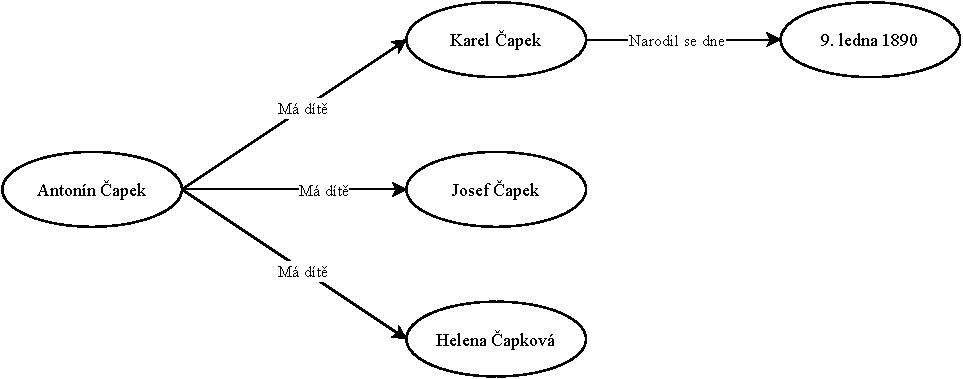
\includegraphics[width=\textwidth]{media/rdf.pdf}
    \caption{Příklad grafu který získáme z předešlých dvou ukázek}
\end{figure}

Pro úplnost zmiňme ještě například následující graf popisující vztahy mezi lidmi, které jsou vyjádřeny ontologií FOAF (friend of a friend). Pokud by všechny zdroje popisující lidi využívali tuto ontologii, měli bychom jednotný interface jak přistupovat k lidským vstahům.

\begin{code}
@prefix foaf: <http://xmlns.com/foaf/0.1/> .
@prefix example: <http://example.org/> .

<http://example.org/Jan-Novák> foaf:name "Jan Novák" .
<http://example.org/Ondřej-Novák> foaf:name "Ondřej Novák" .

example:Pavel-Novotný foaf:name "Pavel Novotný" ;
                      foaf:knows example:Jan-Novák ,
                                 example:Ondřej-Novák .
\end{code}

\subsection{SPARQL jazyk}
Jakyk SPARQL slouží na dotazování nad RDF daty a jejich manipulaci a je použit v definici konfigurací, kde jsou pomocí něj definovány dotazy na získání dalších vrcholů grafu.